\chapter{The NED Language}
\label{cha:the-ned-language}


\section{NED overview}

The description of model topology\index{topology} is given in the NED
language\index{ned!language}. The NED language supports modular
description of a network. This means that a network
description\index{network!description} consists of a number of
component descriptions (channels\index{channel},
simple\index{module!simple}/compound\index{module!compound} module
types). The channels, simple modules and compound
modules of one network description can be reused in another network
description. As a consequence, the NED language makes it possible for
users to build their own module libraries.

Files containing network descriptions generally have a \texttt{.ned}
suffix.  NED files are not used directly: they are
translated into C++ code by the NEDC compiler, then compiled by the
C++ compiler and linked into the simulation executable.

The EBNF description of the language can be found in Appendix
\ref{cha:ned-language-grammar}.


\subsection{Components of a NED description}
\index{ned!components}

A NED description can contain the following components, in arbitrary
number or order:
\begin{itemize}
  \item{import directives\index{import directives}}
  \item{channel definitions\index{channel!definitions}}
  \item{simple\index{module!simple} and compound\index{module!compound} module definitions}
  \item{network definitions\index{network!definitions}}
\end{itemize}


\subsection{Reserved words}
\index{ned!keywords}

The writer of the network description has to take care that no
reserved words are used for names. The reserved words of the
NED language are:
\begin{verbatim}
  import include channel endchannel simple endsimple module endmodule
  error delay datarate const parameters gates submodules connections
  gatesizes on if machines for do endfor network endnetwork nocheck
  ref ancestor true false like input numeric string bool char
\end{verbatim}



\subsection{Case sensitivity}
\index{ned!case sensitivity}

The network description and all identifiers in it are case sensitive.


\subsection{Comments}

\index{ned!comments}

Comments can be placed anywhere in the NED file, with the usual C++
syntax: comments begin with a double slash `//', and last until
the end of the line. Comments are ignored by the NED compiler.

It is planned that future {\opp} versions will use comments
for documentation generation, much like JavaDoc or Doxygen.


\section{The import directive}

\index{ned!import files}
\index{ned!keywords!include}

The \fpar[ned!keywords!import]{import} directive
is used to import declarations from another network description file.
After importing a network description, one can use the components
(channels\index{channel}, simple/compound module types) defined in it.

From the imported files, only the declaration information is used, but
\textit{no C++ code is generated}: you have to compile and link each
network description\index{network!description}, not only the top-level ones.

You can specify the name of the files with or without the
\texttt{.ned} extension. You can also include a path in the
filenames\index{ned!include files}, or better, use the NEDC compiler's
\ttt{-I <path>} command-line option to name the directories where the
imported files reside.

Example:

\begin{Verbatim}[commandchars=\\\{\}]
\tbf{import} "ethernet";   // imports ethernet.ned
\end{Verbatim}




\section{Channel definitions}

\index{channel}
\index{channel!definition}
\index{channel!delay}
\index{channel!error}
\index{channel!datarate}

A channel definition specifies a connection type of given characteristics.
The channel name can be used later in the NED description to
create connections with these parameters.


Example:

\begin{Verbatim}[commandchars=\\\{\}]
\tbf{channel} DialUpConnection
    \tbf{delay} normal (0.004, 0.0018)
    \tbf{error} 0.00001
    \tbf{datarate} 14400
\tbf{endchannel}
\end{Verbatim}

Any of the \fvar{delay}, \fvar{error} and \fvar{datarate} parameters
are optional and they can appear in any order. The values are NED
expressions\index{ned!expressions}.  This means that they can be
constants (integer or real), random values from various distributions,
etc.




\section{Simple module definitions}


Simple modules are the basic building blocks for other (compound)
modules. Simple module types are identified by names.
By convention, module names begin with upper-case letters.

A simple\index{module!simple!definition} module is defined by
declaring its parameters\index{module!parameters} and
gates\index{gate}.

Simple modules are declared with the following syntax:

\begin{Verbatim}[commandchars=\\\{\}]
\tbf{simple} SimpleModuleName
    \tbf{parameters}:
        //...
    \tbf{gates}:
        //...
\tbf{endsimple}
\end{Verbatim}



\subsection{Simple module parameters}
\label{sec:ch-ned-lang:simple-module-param}

\index{module!parameters}

Parameters are variables that belong to a module. Simple module
parameters can be queried and used by simple module algorithms.
For example, a module called \texttt{TrafficGen} may have a parameter
called \ttt{numOfMessages} that determines how many messages it
should generate.

Parameters are identified by names.
By convention, parameter names begin with lower-case letters.

Parameters are declared by listing their names in the
parameters:\index{module!simple!parameter declaration} section of a
module description. The parameter type can optionally be specified as
\fpar[ned!keywords!numeric]{numeric}, \fpar[ned!keywords!numeric const]{numeric const}
(or simply \fpar[ned!keywords!const]{const}),
\fpar[ned!keywords!bool]{bool}, \fpar[ned!keywords!string]{string}, or
\fpar[ned!keywords!anytype]{anytype}.


Example:

\begin{Verbatim}[commandchars=\\\{\}]
\tbf{simple} TrafficGen
    \tbf{parameters}:
        interArrivalTime,
        numOfMessages : \tbf{const},
        address : \tbf{string};
    \tbf{gates}: //...
\tbf{endsimple}
\end{Verbatim}

If the parameter type is omitted, \fpar[ned!keywords!numeric]{numeric}
is assumed. Practically, this means that you only need to explicitly
specify the type for string, bool or char-valued parameters.

Note that the actual parameter values are given later, when the module
is used as a building block of a compound module type or as a system
module.


\textbf{Const parameters}
\label{sec:ch-ned-lang:const}
\index{const}
\index{module!parameters!const}

When you declare a parameter to be \fpar[ned!keywords!const]{const},
it will be evaluated and replaced by the resulting constant value
at the beginning of the simulation. This can be important when the
original value was a random number\index{random!number} or an
expression\index{ned!expression}. One is advised to write out the
\fpar[ned!keywords!const]{const} keyword for each parameter that
should be constant.

Beware when using \fpar[ned!keywords!const]{const} and by-reference
parameter passing (\fpar[ned!keywords!ref]{ref} modifier, see later)
at the same time. Converting the parameter to constant can affect
other modules and cause errors that are difficult to discover.




\subsection{Simple module gates}
\label{sec:ch-ned-lang:simple-module-gates}

\index{gate}
\index{module!simple!gates}

Gates are the connection points of modules. The starting and
ending points of the connections between modules are gates. OMNeT++
supports simplex (one-directional) connections, so there are
two kinds of gates: input and output. Messages are sent through
output gates and received through input gates.

Gates are identified with their names.
By convention, gate names begin with lower-case letters.

Gate vectors are supported: a gate vector\index{gate!vector}
contains a number of single gates.

Gates are declared by listing their names in the
\fpar[ned!keywords!gates]{gates:} section of a module description. An
empty bracket pair [] denotes a gate vector\index{gate!vector}.
Elements of the vector are numbered starting with zero.

Examples:

\begin{Verbatim}[commandchars=\\\{\}]
\tbf{simple} DataLink
    \tbf{parameters}: //...
    \tbf{gates}:
        \tbf{in}:  fromPort, fromHigherLayer;
        \tbf{out}: toPort, toHigherLayer;
\tbf{endsimple}

\tbf{simple} RoutingModule
    \tbf{parameters}: //...
    \tbf{gates}:
        \tbf{in}:  output[];
        \tbf{out}: input[];
\tbf{endsimple}
\end{Verbatim}

The sizes of gate vectors are given later, when the module is used as
a building block of a compound module type. Thus, every instance of
the module can have gate vectors of different sizes.





\section{Compound module definitions}


Compound modules are modules composed of one or more submodules.
Any module type (simple or compound module) can be used as a submodule.
Like simple modules, compound modules can also have gates and parameters,
and they can be used wherever simple modules can.

It is useful to think about compound modules as ``cardboard boxes''
that help you organize your simulation model and bring structure into
it. No active behaviour is associated with compound modules -- they
are simply for grouping modules into larger components that can
can be used either as a model (see section \ref{sec:ch-ned-lang:network})
or as a building block for other compound modules.

By convention, module type names (and so compound module type names, too)
begin with upper-case letters.

Submodules may use parameters of the compound module.
They may be connected with each other and/or with
the compound module itself.

A compound module definition\index{module!compound!definition} looks
similar to a simple\index{module!simple} module definition:
it has \texttt{gates} and \texttt{parameters} sections.
There are two additional sections, \texttt{submodules} and
\texttt{connections}.

The syntax for compound modules is the following:

\begin{Verbatim}[commandchars=\\\{\}]
\tbf{module} CompoundModule
    \tbf{parameters}:
        //...
    \tbf{gates}:
        //...
    \tbf{submodules}:
        //...
    \tbf{connections}:
        //...
\tbf{endmodule}
\end{Verbatim}

All sections (\texttt{parameters}, \texttt{gates}, \texttt{submodules},
\texttt{connections}) are optional.



\subsection{Compound module parameters and gates}

Parameters\index{module!compound!parameters} and gates \index{gate}
for compound modules are declared and work in the same way
as with simple modules, described in sections
\ref{sec:ch-ned-lang:simple-module-param}
and \ref{sec:ch-ned-lang:simple-module-gates}.

Typically, compound module parameters are passed to submodules and
used for initializing their parameters.

Parameters can also be used in defining the internal structure of
the compound module: the number of submodules, gate vector sizes
can be define with the help of parameters, and parameters can
also be used in defining the connections inside the compound module.
As a practical example, you can create a \ttt{Router} compound module
with a variable number of ports, specified in a \ttt{numOfPorts} parameter.

Parameters affecting the internal structure should always be declared
\ttt{const}, so that accessing them always yields the same value.
(Otherwise, if the parameter was assigned a random value, one could
get a different value each time the parameter is accessed during building
the internals of the compound module, which is surely not what was meant.)

Example:

\begin{Verbatim}[commandchars=\\\{\}]
\tbf{module} Router
    \tbf{parameters}:
        packetsPerSecond : \tbf{numeric},
        bufferSize : \tbf{numeric},
        numOfPorts : \tbf{const};
    \tbf{gates}:
        \tbf{in}: inputPort[];
        \tbf{out}: outputPort[];
    \tbf{submodules}: //...
    \tbf{connections}: //...
\tbf{endmodule}
\end{Verbatim}


\subsection{Submodules}

Submodules\index{module!submodule} are defined in the
\fpar[ned!keywords!submodules]{submodules:} section of a compound
module declaration. Submodules are identified by names.
By convention, submodule names begin with lower-case letters.

Submodules are instances of a module type, either simple
or compound -- there is no distinction. The module type
must be known to the NED compiler, that is, it must have appeared
earlier in the same NED file or have been imported from another
NED file.

It is possible to define vectors of submodules, and the
size of the vector may come from a parameter value.

When defining submodules, you can assign values to their
parameters, and if the corresponding module type has gate vectors,
you have to specify their sizes.


Example:

\begin{Verbatim}[commandchars=\\\{\}]
\tbf{module} CompoundModuleName
    //...
    \tbf{submodules}:
        submodule1: ModuleType1
            \tbf{parameters}:
                //...
            \tbf{gatesizes}:
                //...
        submodule2: ModuleType2
            \tbf{parameters}:
                //...
            \tbf{gatesizes}:
                //...
\tbf{endmodule}
\end{Verbatim}


\tbf{Module vectors}


It is possible to create an array\index{module!array} of
submodules\index{submodule|see{module}} (a module
vector\index{module!vector}).  This is done with an expression between
brackets right behind the module type name. The expression can refer
to module parameters. A zero value as module count is also allowed.

Example:

\begin{Verbatim}[commandchars=\\\{\}]
\tbf{module} BigCompoundModule
    \tbf{parameters}:
        size: \tbf{const};
    \tbf{submodules}:
        submod1: Node[3]
            //...
        submod2: Node[size]
            //...
        submod3: Node[2*size+1]
            //...
\tbf{endmodule}
\end{Verbatim}



\subsection{Submodule type as parameter}
\label{sec:ch-ned-lang:like}
\index{module!as parameter}

Sometimes it is convenient to make the type of a submodule
to be a parameter, so that you can easily ``plug in''
any module type there.

For example, assume the purpose of your simulation study is
to compare different routing algorithms. Suppose you programmed
the needed routing algorithms as simple modules: \texttt{DistVecRoutingNode},
\texttt{AntNetRouting1Node}, \texttt{AntNetRouting2Node}, etc.
You have also created the network topology as a compound module
called \ttt{RoutingTestNetwork}, which will serve as a testbed for your routing
algorithms. Currently, \ttt{RoutingTestNetwork} has \texttt{DistVecRoutingNode}
hardcoded (all submodules are of this type), but you want
to be able to switch to other routing algorithms easily.

NED gives you the possibility to add a string-valued parameter,
say \ttt{routingNodeType} to the \ttt{RoutingTestNetwork} compound module.
Then you can tell NED that types of the submodules inside \ttt{RoutingTestNetwork}
are not of any fixed module type, but contained in the \ttt{routingNodeType}
parameter. That's all -- now you are free to assign any of
the \texttt{"DistVecRoutingNode"}, \texttt{"AntNetRouting1Node"} or
\texttt{"AntNetRouting2Node"} string constants to this parameter
(you can do that in NED, in the config file (\ttt{omnetpp.ini}),
or even enter in interactively),
and your network will use the routing algorithm you chose.

If you specify a wrong value, say \texttt{"FooBarRoutingNode"}
whereas you have no \ttt{FooBarRoutingNode} module implemented,
you'll get a runtime error at the beginning of the simulation:
\textit{module type definition not found}.

Inside the \ttt{RoutingTestNetwork} module you assign parameter values
and connect the gates of the routing modules. To provide some degree
of type safety, NED wants to make sure you didn't misspell
parameter or gate names and you used them correctly.
To be able to do such checks, NED requires some help from you: 
you have to name an existing module type (say \ttt{RoutingNode})
and promise NED that all modules you're going you specify
in the \ttt{routingNodeType} parameter will have (at least) the same
parameters and gates as the \ttt{RoutingNode} module.
  \footnote{If you like, the above solution somewhat similar to polymorphism
  in object-oriented languages -- \ttt{RoutingNode} is like a
  ``base class'', \texttt{DistVecRoutingNode} and \texttt{AntNetRouting1Node}
  are like ``derived classes'', and the \ttt{routingNodeType} parameter
  is like a ``pointer to a base class'' which may be downcast to specific
  types.}

All the above is achieved via the \fpar[ned!keywords!like]{like} keyword.
The syntax is the following:

\begin{Verbatim}[commandchars=\\\{\}]
\tbf{module} RoutingTestNetwork
    \tbf{parameters}:
        routingNodeType: \tbf{string}; // should hold the name
                                  // of an existing module type
    \tbf{gates}: //...
    \tbf{submodules}:
        node1: routingNodeType \tbf{like} RoutingNode;
        node2: routingNodeType \tbf{like} RoutingNode;
        //...
    \tbf{connections nocheck}:
        node1.out0 --> node2.in0;
        //...
\tbf{endmodule}
\end{Verbatim}

The \texttt{RoutingNode} module type does not need to be implemented in
C++, because no instance of it is created; it is merely used
to check the correctness of the NED file.

On the other hand, the actual module types that will be substituted
(e.g. \texttt{DistVecRoutingNode}, \texttt{AntNetRouting1Node},etc.)
do not need to be declared in the NED files.

The \fpar[ned!keywords!like]{like} phrase lets you create families
of modules that serve similar purposes and implement the same interface
(they have the same gates and parameters)
and to use them interchangeably in NED files.




\subsection{Assigning values to submodule parameters}

\index{module!submodule!parameters}

If the module type used as submodule has parameters, you can assign
values to them in the \texttt{parameters} section of the submodule
declaration.
As a value you can use a constant (such as \texttt{42} or
\texttt{"www.foo.org"}), various parameters (most commonly, parameters
of the compound module), or write an arbitrary expression containing
the above.

It is not mandatory to mention and assign all parameters.
Unassigned parameters can get their values at runtime: either from
the configuration file (\texttt{omnetpp.ini}), or if the value
isn't there either, the simulator will prompt you to enter it
interactively. Indeed, for flexibility reasons it is often very useful
not to ``hardcode'' parameter values in the NED file,
but to leave them to \texttt{omnetpp.ini} where they can be
changed more easily.


Example:

\begin{Verbatim}[commandchars=\\\{\}]
\tbf{module} CompoundModule
    \tbf{parameters}:
        param1: numeric,
        param2: numeric,
        useParam1: bool;
    \tbf{submodules}:
        submodule1: Node
            \tbf{parameters}:
                p1 = 10,
                p2 = param1+param2,
                p3 = useParam1==true ? param1 : param2;
        //...
\tbf{endmodule}
\end{Verbatim}


The expression syntax \index{ned!expressions} is very similar to C.
Expressions may contain constants (literals) and parameters of the
compound module being defined. Parameters can be passed by value
or by reference. The latter means that the expression is evaluated
at runtime each time its value is accessed (e.g. from simple module
code), opening up interesting possibilities for the modeler.
You can also refer to parameters of the already defined submodules,
with the syntax \ttt{submodule.parametername}
(or \ttt{submodule[index].parametername}).

Expressions are described in detail in section \ref{ch-ned-lang:sec:expressions}.


\textbf{The \ttt{input} keyword}
\label{sec:ch-ned-lang:input}

When a parameter does not receive a value inside NED files or in
the configuration file (\ttt{omnetpp.ini}), the user will be prompted
to enter its value at the beginning of the simulation.
If you plan to make use of interactive prompting, you can specify
a prompt text and a default value.

The syntax is the following:

\begin{Verbatim}[commandchars=\\\{\}]
    \textit{<paramname>} = \tbf{input}(\textit{<default-value>}, \textit{<prompt>})
    \textit{<paramname>} = \tbf{input}(\textit{<default-value>})
    \textit{<paramname>} = \tbf{input}
\end{Verbatim}

The third version is actually equivalent to simply and quietly
leaving out the parameter from the list of assignments, but
you can use it to make it explicit that you do not want to
assign a value from within the NED file.

Examples:

\begin{Verbatim}[commandchars=\\\{\}]
   parameters:
      numProc = \tbf{input}(10, "Number of processors?"),
      processingTime = \tbf{input}(10ms);
\end{Verbatim}



\subsection{Defining sizes of submodule gate vectors}

\index{module!gate sizes}
\index{gate!vector!size}

The sizes of gate vectors are defined with the
\fpar[ned!keywords!gatesizes]{gatesizes} keyword.  Gate vector sizes
can be given as constants, parameters or expressions.

An example:

\begin{Verbatim}[commandchars=\\\{\}]
\tbf{simple} Node
    \tbf{gates}:
        \tbf{in}: inputs[];
        \tbf{out}: outputs[];
\tbf{endsimple}

\tbf{module} CompoundModule
    \tbf{parameters}:
        numPorts: \tbf{const};
    \tbf{submodules}:
        node1: Node
            \tbf{gatesizes}:
                inputs[2], outputs[2];
        node2: Node
            \tbf{gatesizes}:
                inputs[numPorts], outputs[numPorts];
        //...
\tbf{endmodule}
\end{Verbatim}


\subsection{Conditional parameters and gatesizes sections}


Multiple \ttt{parameters}\index{ned!parameters} and
\texttt{gatesizes}\index{ned!gatesizes} sections can exist in a submodule
definition and each of them can be tagged with
conditions\index{gate!conditional}.

Example:

\begin{Verbatim}[commandchars=\\\{\}]
\tbf{module} Tandem
    \tbf{parameters}: count: \tbf{const};
    \tbf{submodules}:
        node : Node [count]
            \tbf{parameters}:
                position = "middle";
            \tbf{parameters} \tbf{if} index==0:
                position = "beginning";
            \tbf{parameters} \tbf{if} index==count-1:
                position = "end";
            \tbf{gatesizes}:
                in[2], out[2];
            \tbf{gatesizes} \tbf{if} index==0 {\textbar}{\textbar} index==count-1:
                in[1], in[1];
    \tbf{connections}:
        //...
\tbf{endmodule}
\end{Verbatim}


If the conditions are not disjoint and a parameter value or a
gate size is defined twice, the last definition will take effect,
overwriting the former ones. Thus, values intended as defaults
should appear in the first sections.



\subsection{Connections}


The compound module definition specifies how the gates of the compound
module and its immediate sub-modules are connected\index{connection}.

You can connect two submodules or a submodule with its enclosing
compound module. (For completeness, you can also connect two gates
of the compound module on the inside, but this is rarely needed).
This means that NED does not permit connections that span
multiple levels of hieararchy -- this restriction
enforces compound modules to be self-contained, and thus promotes
reusability. Gate directions must also be observed,
that is, you cannot connect two output gates or two input gates.

Only one-to-one connections are supported. One-to-many and many-to-one
connections can be achieved using simple modules that duplicate
messages or merge message flows. The rationale is that wherever
such fan-in or fan-out occurs in a model, it is usually associated
with some processing anyway that makes it necessary to use
simple modules.

A gate can only be connected once: if two connections refer to
the same gate, a compilation or runtime error will occur.

By default, NED expects every gate to be connected, resulting in
a compilation or runtime error if an unconnected gate is found.
This check can be turned off with the \ttt{nocheck} modifier,
described later in this section.

Connections\index{ned!connections} are specified in the
\fpar[ned!keywords!connections]{connections:} section of a compound
module definition. It lists the connections, separated by semicolons.

Example:

\begin{Verbatim}[commandchars=\\\{\}]
\tbf{module} CompoundModule
    \tbf{parameters}: //...
    \tbf{gates}: //...
    \tbf{submodules}: //...
    \tbf{connections}:
        node1.output --> node2.input;
        node1.input <-- node2.output;
        //...
\tbf{endmodule}
\end{Verbatim}


Each connection can be:
\begin{itemize}
  \item{simple (that is, no delay, bit error rate or data rate), can
    use a named channel, or a channel given with delay, error and
    data rate values;}
\item{single or multiple (loop) connection;}
\item{conditional or non-conditional.}
\end{itemize}

These connection types are described in the following sections.


\tbf{Single connections and channels}

\index{ned!connections}
\index{connection}

The source gate can be an output gate of a submodule or an input
gate of the compound module, and the destination gate can be
an input gate of a submodule or an output gate of the compound
module.


If you do not specify a channel\index{channel}, the connection will have
no propagation delay, no transmission delay and no bit errors:
\begin{verbatim}
    sender.outGate --> receiver.inGate;
\end{verbatim}

The arrow can point either left-to-right or right-to-left.

You can specify a channel by its name\index{channel!name}:
\begin{verbatim}
    sender.outGate --> Dialup14400 --> receiver.inGate;
\end{verbatim}

In this case, the NED sources must contain the definition of
the channel.

One can also specify the channel parameters directly\index{channel!parameters}:
\begin{verbatim}
    sender.outGate --> error 1e-5 delay 0.001 --> receiver.inGate;
\end{verbatim}

Either of the parameters can be omitted and they can be in any
order.


\tbf{Loop connections}


If submodule or gate vectors are used, it is possible to create
more than one connection with one statement. This is termed a \textit{multiple}
or \textit{loop connection}\index{connection!loop}.

A multiple connection is created with the \fpar[ned!keywords!for]{for}
statement:

\begin{Verbatim}[commandchars=\\\{\}]
\tbf{for} i=0..4 \tbf{do}
    sender.outGate[i] --> receiver[i].inGate
\tbf{endfor};
\end{Verbatim}


The result of the above loop connection can be illustrated as
depicted in Fig. \ref{fig:ch-ned-lang:loop-connection}.

\begin{figure}[htbp]
\begin{center}
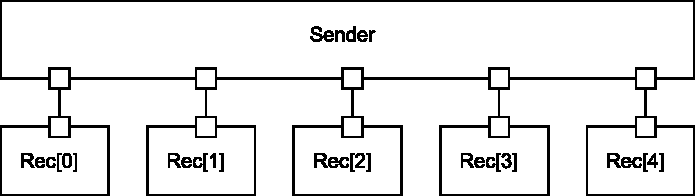
\includegraphics[width=4.625in, height=1.297in]{figures/usmanFig7}
\caption{Loop connection}
\label{fig:ch-ned-lang:loop-connection}
\end{center}
\end{figure}


One can place several connections in the body of the
\fpar[ned!keywords!for]{for} statement, separated by semicolons.

One can create nested loops\index{ned!nested for statements}
by specifying more than one indices in the \texttt{for} statement,
with the first variable forming the outermost loop.

\begin{Verbatim}[commandchars=\\\{\}]
\tbf{for} i=0..4, j=0..4 \tbf{do}
    //...
\tbf{endfor};
\end{Verbatim}

One can also use an index in the lower and upper bound expressions
of the subsequent indices:

\begin{Verbatim}[commandchars=\\\{\}]
\tbf{for} i=0..3, j=i+1..4 \tbf{do}
    //...
\tbf{endfor};
\end{Verbatim}


\tbf{Conditional connections}

\index{connection!conditional}

Creation of a connection can be made conditional, using the \ttt{if}
keyword:

\index{ned!keywords!if}

\begin{Verbatim}[commandchars=\\\{\}]
\tbf{for} i=0..n \tbf{do}
    sender.outGate[i] --> receiver[i].inGate \tbf{if} i\%2==0;
\tbf{endfor};
\end{Verbatim}

The \ttt{if} condition is evaluated for each connection
(in the above example, for each \textit{i} value), and the
decision is made individually each time whether to create the
the connection or not. In the above example we connected every
second gate. Conditions may also use random variables, as
shown in the next section.


\tbf{The nocheck modifier}

By default, NED requires that all gates be connected. Since this
check can be inconvenient at times, it can be turned off
using the \fpar[ned!keywords!nocheck]{nocheck} modifier.

The following example generates a random subgraph of a full graph.

\begin{Verbatim}[commandchars=\\\{\}]
\tbf{module} RandomConnections
    \tbf{parameters}: //..
    \tbf{gates}: //..
    \tbf{submodules}: //..
    \tbf{connections} \tbf{nocheck}:
        \tbf{for} i=0..n-1, j=0..n-1 \tbf{do}
            node[i].out[j] --> node[j].in[i] \tbf{if} uniform(0,1)<0.3;
        \tbf{endfor};
\tbf{endmodule}
\end{Verbatim}

When using \fpar[ned!keywords!nocheck]{nocheck}, it is the
simple modules' responsibility not to send messages on gates
that are not connected.


\section{Network definitions}
\label{sec:ch-ned-lang:network}
\index{ned!network definition}

Module module declarations (compound and simple module declarations)
just define module types. To actually get a simulation model that
can be run, you need to write a \textit{network definition}.

A network definition declares a simulation model as an instance
of a previously defined module type. You'll typically want to use
a compound module type here, although it is also possible to
program a model as a self-contained simple module and instantiate it
as a ``network''.

There can be several network definitions in your NED file or NED files.
The simulation program that uses those NED files will be
able to run any of them; you typically select the desired one
in the config file (\ttt{omnetpp.ini}).

The syntax of a network definition is similar that of a submodule
declaration:

\begin{Verbatim}[commandchars=\\\{\}]
\tbf{network} wirelessLAN: WirelessLAN
    \tbf{parameters}:
        numUsers=10,
        httpTraffic=true,
        ftpTraffic=true,
        distanceFromHub=truncnormal(100,60);
\tbf{endnetwork}
\end{Verbatim}

Here, \ttt{WirelessLAN} is the name of previously defined
compound module type, which presumably contains further
compound modules of types \ttt{WirelessHost}, \ttt{WirelessHub}, etc.

Naturally, only compound module types without gates can
be used in network definitions.

Just as for submodules, you do not need to assign values to all
parameters. Unassigned parameters will get their values from the
config file (\ttt{omnetpp.ini}) or interactively prompted for.



\section{Expressions}
\label{ch-ned-lang:sec:expressions}

In the NED language there are a number of places where
expressions\index{ned!expressions} are expected.

Expressions have a C-style syntax. They are built with the usual math
operators\index{math operators}; they can use parameters taken by
value or by reference; call C functions; contain random and input
values etc.

When an expression is used for a parameter value, it is evaluated
each time the parameter value is accessed (unless the parameter is
declared \ttt{const}, see \ref{sec:ch-ned-lang:const}). This means
that a simple module querying a non-const parameter during simulation
may get different values each time (e.g. if the value involves a
random variable, or it contains other parameters taken by reference).
Other expressions (including \ttt{const} parameter values)
are evaluated only once.


\subsection{Constants}

\textbf{Numeric and string constants}

Numeric constants are accepted in their usual decimal or
scientific notations.

%% FIXME Only decimal notation is accepted!!! no hex, octal or binary...

\textbf{String constants}

String constants use double quotes.

%% FIXME no escape character sequences are accepted!!!

\textbf{Time constants}

Anywhere you would put numeric constants\index{numeric constants}
(integer or real) to mean time in seconds, you can also specify the
time in units like milliseconds, minutes or hours:


\begin{Verbatim}[commandchars=\\\{\}]
    ...
    \tbf{parameters}:
        propagationDelay = 560ms, // 0.560s
        connectionTimeout = 6m 30s 500ms, // 390.5s
        recoveryIntvl = 0.5h; // 30 min
\end{Verbatim}


The following units\index{time units} can be used:

\begin{longtable}{|c|l|l|}
\hline
\tabheadcol
\tbf{Unit} & \tbf{Meaning} & \tbf{Seconds} \\\hline
\ttt{ns} & nanoseconds & $*10^{-9}$ \\\hline
\ttt{us} & microseconds & $*10^{-6}$ \\\hline
\ttt{ms} & milliseconds & $*10^{-3}$ \\\hline
\ttt{s}  & seconds & $*1$ \\\hline
\ttt{m}  & minutes & $*60$ \\\hline
\ttt{h}  & hours & $*3600$ \\\hline
\ttt{d}  & days & $*24*3600$ \\\hline
\end{longtable}


\subsection{Referencing parameters}

Expressions can use the parameters of the enclosing compound module
(the one being defined) and of submodules defined earlier in NED file.
The syntax for the latter is \ttt{submod.param} or \ttt{submod[index].param}.

You can refer to a compound module parameter called \ttt{param}
in several ways: as \ttt{param}, \ttt{\textbf{ref} param},
\ttt{\textbf{ancestor} param}, or \ttt{\textbf{ref} \textbf{ancestor} param}.
They all have different semantics.

The first two variations, \ttt{param} and \ttt{\textbf{ref} param}
lets you access the parameters of the compound module being
defined. In the third and fourth versions, the keyword
\ttt{ancestor} means that the parameter will be searched for upwards,
in the module nesting hierarchy. Naturally, this kind of reference can
only be resolved at runtime, when the whole network has been built up.
The parameter which is found first is used. If no such parameter can be
found in any of the enclosing modules, it is a runtime error.

The \ttt{ref} and \ttt{ref}-less versions differ in how the parameter
is taken: by value or by reference. If you take a parameter by reference,
then runtime changes to that parameter will be reflected in the
assigned parameter: each time a simple module reads the parameter
value, the expression is evaluated, and you may get a different value.
In contrast, if you take the parameter by value, then runtime changes
do not affect the assigned parameter.
  \footnote{This also means that if an expression doesn't contain any parameter
  taken by reference, the NED compiler may have the possibility to evaluate
  the expression only once, at compile time. If an expression refers
  to parameters taken by reference, only runtime evaluation can be used.}

Reference parameters open up interesting possibilities for the modeler.
For example, you can define a parameter that at the highest level
of the model, and let other modules take it by reference --
then if you change the parameter value at runtime
(manually or from a simple module), it will affect the whole model.
You can use this arrangement to ``tune'' model parameters at runtime,
in search for an optimal setting.

In another setup, reference parameters can be used by to propagate
status values to neighbouring modules.



\subsection{Operators}

The set of operators supported in NED is similar to C/C++\index{ned!expressions!operators},
with the following differences:

\begin{itemize}
  \item{{\textasciicircum} is used for power-of (and not bitwise XOR as in C)}
  \item{\# is used for logical XOR (same as != between logical values), and
        \#\# is used for bitwise XOR}
  \item{the precedence of bitwise operators (\&, |, \#) have been raised
        to bind stronger than relational operations. This precedence is usually 
        more convenient than the C/C++ one.}
\end{itemize}

All values are represented as \ttt{double}s. For the bitwise operators,
\ttt{double}s are converted to \ttt{unsigned long}
  \footnote{In case you are worried about \ttt{long} values being not accurately
  represented in \ttt{double}s, this is not the case. IEEE-754 \ttt{double}s
  have 52 bit mantissas, and integer numbers in that range are represented
  without rounding errors.}
using the C/C++ builtin conversion (type cast), the operation is performed,
then the result is converted back to \ttt{double}.
Similarly, for the logical operators \&\&, || and \#\#,
the operands are converted to \ttt{bool} using the C/C++ builtin
conversion (type cast), the operation is performed, then the result
is converted back to \ttt{double}. For modulus (\%), the operands are
converted to \ttt{long}.

Here's the complete list of operators, in order of decreasing precendence:

\begin{longtable}{|l|l|}
\hline
\tabheadcol
\tbf{Operator}          & \tbf{Meaning} \\\hline
%%
-, !, \ensuremath{\sim} & unary minus, negation, bitwise complement \\\hline
%%
{\textasciicircum}      & power-of \\\hline
%%
$*$, /, \%              & multiply, divide, modulus \\\hline
%%
+, -                    & add, subtract \\\hline
%%
\ttt{<<}, \ttt{>>}      & bitwise shifting \\\hline
%%
\&, |, \#               & bitwise and, or, xor \\\hline
%%
==                      & equal \\
!=                      & not equal \\
\ttt{>}, \ttt{>=}       & greater, greater or equal \\
\ttt{<}, \ttt{<=}       & less, less or equal \\\hline
%%
\&\&, ||, \#\#          & logical operators and, or, xor \\\hline
%%
?:                      & the C/C++ ``inline if'' \\\hline
\end{longtable}



\subsection{The \fname{sizeof()} and \fname{index} operators}

A useful operator is \fname{sizeof()}\index{ned!sizeof()}, which gives the
size of a vector gate\index{gate!vector}. The \fname{index}
operator\index{ned!index operator} gives the index of the current
submodule in its module vector.

An example for both:

\begin{Verbatim}[commandchars=\\\{\}]
\tbf{module} Compound
    \tbf{gates}: \tbf{in}: fromgens[];
    \tbf{submodules}:
        proc: Processor[ \tbf{sizeof}(fromgens) ];
            \tbf{parameters}: address = 10*(1+\tbf{index});
    \tbf{connections}:
        \tbf{for} i = 0.. \tbf{sizeof}(fromgens)-1 \tbf{do}
            in[i] --> proc[i].input;
        \tbf{endfor};
\tbf{endmodule}
\end{Verbatim}


Here, we create as many processors as there are input gates for
this compound module in the network. The address parameters of
the processors are 10, 20, 30 etc.




\subsection{Functions}
\index{ned!functions}

In NED expressions, you can use the following mathematical functions:
\begin{itemize}
  \item{many of the C language's \ttt{<math.h>} library functions:
    \ttt{exp()}, \ttt{log()}, \ttt{sin()}, \ttt{cos()}, \ttt{floor()},
    \ttt{ceil()}, \ttt{etc.}}
  \item{functions that generate random variables: \ttt{uniform},
    \ttt{exponential}, \ttt{normal} and others were already
    discussed.}
\end{itemize}

It is possible to add new ones, see \ref{sec:ch-ned-lang:defining-functions}.

\subsection{Random values}

Expressions may contain random variates from different distributions.
This has the effect that unless the parameter was declared \ttt{const},
it returns a different value each time it is evaluated.

If the parameter \textit{was} declared \ttt{const}, it is only evaluated
once at the beginning of the simulation, and subsequent queries
on the parameter will always return the same value.

Random variate functions use one of the random number generators (RNGs)
provided by \opp. By default this is generator 0, but you can specify
which one to be used.

{\opp} has the following predefined distributions\index{distribution!predefined}:

\begin{longtable}{|p{6.5cm}|p{7.5cm}|}
\hline
\tbf{Function} & \tbf{Description}\\\hline
\multicolumn{2}{|c|}{\tbf{Continuous distributions}}\\\hline
\fname{uniform(a, b, \textit{rng=0})} & uniform distribution in the range [a,b) \\\hline
\fname{exponential(mean, \textit{rng=0})} & exponential distribution with the given mean \\\hline
\fname{normal(mean, stddev, \textit{rng=0})} & normal distribution with the given mean and standard deviation \\\hline
\fname{truncnormal(mean, stddev, \textit{rng=0})} & normal distribution truncated to nonnegative values \\\hline
\fname{gamma\_d(alpha, beta, \textit{rng=0})} & gamma distribution with parameters alpha>0, beta>0 \\\hline
\fname{beta(alpha1, alpha2, \textit{rng=0})} & beta distribution with parameters alpha1>0, alpha2>0 \\\hline
\fname{erlang\_k(k, mean, \textit{rng=0})} & Erlang distribution with k>0 phases and the given mean \\\hline
\fname{chi\_square(k, \textit{rng=0})} & chi-square distribution with k>0 degrees of freedom \\\hline
\fname{student\_t(i, \textit{rng=0})} & student-t distribution with i>0 degrees of freedom \\\hline
\fname{cauchy(a, b, \textit{rng=0})} & Cauchy distribution with parameters a,b where b>0 \\\hline
\fname{triang(a, b, c, \textit{rng=0})} & triangular distribution with parameters a<=b<=c, a!=c \\\hline
\fname{lognormal(m, s, rng=0)} & lognormal distribution with mean m and variance s>0 \\\hline
\fname{weibull(a, b, \textit{rng=0})} & Weibull distribution with parameters a>0, b>0 \\\hline
\fname{pareto\_shifted(a, b, c, \textit{rng=0})} & generalized Pareto distribution with parameters a, b and shift c \\\hline
\multicolumn{2}{|c|}{\tbf{Discrete distributions}} \\\hline
\fname{intuniform(a, b, \textit{rng=0})} & uniform integer from a..b \\\hline
\fname{bernoulli(p, \textit{rng=0})} & result of a Bernoulli trial with probability 0<=p<=1 (1 with probability p and 0 with probability (1-p)) \\\hline
\fname{binomial(n, p, \textit{rng=0})} & binomial distribution with parameters n>=0 and 0<=p<=1 \\\hline
\fname{geometric(p, \textit{rng=0})} & geometric distribution with parameter 0<=p<=1 \\\hline
\fname{negbinomial(n, p, \textit{rng=0})} & binomial distribution with parameters n>0 and 0<=p<=1\\\hline
\fname{poisson(lambda, \textit{rng=0})} & Poisson distribution with parameter lambda \\\hline

\end{longtable}

%
% FIXME insert this into the table then hypergeom() starts to work:
% fname{hypergeometric(a, b, n, \textit{rng=0})} & hypergeometric distribution with parameters a>0,b>0 and 0<=n<=a+b.\\\hline
%

If you do not specify the optional \fpar{rng} argument, the functions will
use random number generator 0.

Examples:

\begin{verbatim}
intuniform(0,10)/10  // one of: 0, 0.1, 0.2, ..., 0.9, 1
exponential(5)       // exponential with mean=5 (thus parameter=0.2)
2+truncnormal(5,3)   // normal distr with mean 7 truncated to >=2 values
\end{verbatim}

The above distributions are implemented with C functions, and you can easily
add new ones (see section \ref{sec:ch-ned-lang:defining-functions}).
Your distributions will be treated in the same way as the built-in ones.



\subsection{Defining new functions}
\index{ned!functions}
\label{sec:ch-ned-lang:defining-functions}

To use user-defined functions\index{functions!user-defined}, one has
to code the function in C++.  The C++ function must take 0, 1, 2, 3, or 4
arguments of type double and return a double. The function must be
registered in one of the C++ files with the \fmac{Define\_Function()}
macro.

An example function (the following code must appear in one of the C++
sources):


\begin{verbatim}
#include <omnetpp.h>

double average(double a, double b)
{
  return (a+b)/2;
}

Define_Function(average, 2);
\end{verbatim}


The number 2 means that the \fname{average()} function has 2
arguments.  After this, the \fname{average()} function can be used in
NED files:


\begin{Verbatim}[commandchars=\\\{\}]
\tbf{module} Compound
    \tbf{parameter}: a,b;
    \tbf{submodules}:
        proc: Processor
            \tbf{parameters}: av = average(a,b);
\tbf{endmodule}
\end{Verbatim}


If your function takes parameters that are \ttt{int} or \ttt{long} or
some other type which is not \ttt{double}, you can create wrapper function
that takes all doubles and does the conversion. In this case you have
to register the wrapper function with the \fname{Define\_Function2()} macro
which allows a function to be registered with a name different from the
name of the function that implements it. You can do the same
if the return value differs from \ttt{double}.

\begin{verbatim}
#include <omnetpp.h>

long factorial(int k)
{
  ...
}

static double _wrap_factorial(double k)
{
  return factorial((int)k);
}

Define_Function2(factorial, _wrap_factorial, 1);
\end{verbatim}



\section{Display strings}
\label{sec:ch-ned-lang:display-strings}


Display strings\index{display strings} specify the arrangement and
appearance of modules in graphical user interfaces (currently only
Tkenv): they control how the objects (compound modules, their
submodules and connections) are displayed. Display strings occur in
NED description's \fpar[ned!keywords!display]{display:}
phrases.

The display string format is a semicolon-separated list of tags.
Each tag consists of a key (usually one letter), an equal sign
and a comma-separated list of parameters, like:

\begin{verbatim}
  "p=100,100;b=60,10,rect;o=blue,black,2"
\end{verbatim}

Parameters may be omitted also at the end and also inside the
parameter list, like:

\begin{verbatim}
  "p=100,100;b=,,rect;o=blue,black"
\end{verbatim}

Module/submodule parameters can be included with the \ttt{\$name} notation:

\begin{verbatim}
  "p=$xpos,$ypos;b=rect,60,10;o=$fillcolor,black,2"
\end{verbatim}
%%$

Objects that may have display strings are:
\begin{itemize}
  \item{compound modules (as the enclosing module in the drawing),}
  \item{submodules}
  \item{connections}
\end{itemize}



\subsection{Submodule display strings}


The following table lists the tags used in submodule display strings:

\index{display strings!tags}

\begin{longtable}{|p{6cm}|p{8cm}|}
\hline
% ROW 1
\tabheadcol
\tbf{Tag} & \tbf{Meaning} \\\hline
% ROW 2
\tbf{p=}\textit{xpos},\textit{ypos}
&
{\raggedright Place submodule at (\textit{xpos},\textit{ypos}) pixel position,
with the origin being the top-left corner of the enclosing module.

Defaults: an appropriate automatic layout is where submodules do not overlap.

If applied to a submodule vector, \textit{ring} or \textit{row} layout is
selected automatically.}\\\hline
% ROW 3
\tbf{p=}\textit{xpos},\textit{ypos},\tbf{row},\textit{deltax} &
{\raggedright Used for module vectors. Arranges submodules in a row starting
at (\textit{xpos},\textit{ypos}), keeping \textit{deltax} distances.

Defaults: \textit{deltax} is chosen so that submodules do not overlap.

\tbf{row} may be abbreviated as \tbf{r}.}\\\hline
% ROW 4
\tbf{p=}\textit{xpos},\textit{ypos},\tbf{column},\textit{deltay}
&
{\raggedright Used for module vectors. Arranges submodules in a column starting
at (\textit{xpos},\textit{ypos}), keeping \textit{deltay} distances.

Defaults: \textit{deltay} is chosen so that submodules do not overlap.

\tbf{column} may be abbreviated as \tbf{col} or \tbf{c}.}\\\hline
% ROW 5
\tbf{p=}\textit{xpos},\textit{ypos},\tbf{matrix},
\textit{itemsperrow},\textit{deltax},\textit{deltay}
&
{\raggedright Used for module vectors. Arranges submodules in a matrix starting
at (\textit{xpos},\textit{ypos}), at most \textit{itemsperrow} submodules in
a row, keeping \textit{deltax} and \textit{deltay} distances.

Defaults: \textit{itemsperrow}=5, \textit{deltax,deltay} are chosen so that
submodules do not overlap.

\tbf{matrix} may be abbreviated as \tbf{m}.}\\\hline
% ROW 6
\tbf{p=}\textit{xpos},\textit{ypos},\tbf{ring},\textit{width,height}
&
{\raggedright Used for module vectors. Arranges submodules in an ellipse,
with the top-left corner of its bounding boxes at (\textit{xpos},\textit{ypos}),
with the \textit{width} and \textit{height}.

Defaults: \textit{width}=40, \textit{height}=24

\tbf{ring} may be abbreviated as \tbf{ri}.}\\\hline
% ROW 7
\tbf{p=}\textit{xpos},\textit{ypos},\tbf{exact},\textit{deltax},\textit{deltay}
&
{\raggedright Used for module vectors. Each submodule is placed at
\textit{(xpos+deltax}, \textit{ypos+deltay)}.
This is useful if \textit{deltax} and \textit{deltay} are parameters
 (e.g.:\textit{''p=100,100,exact,\$x,\$y''})
which take different values for each module in the vector.

Defaults: \textit{none}

\tbf{exact} may be abbreviated as \tbf{e} or \tbf{x}.}\\\hline
% ROW 8
\tbf{b=}\textit{width},\textit{height},\tbf{rect}
&
{\raggedright Rectangle with the given \textit{height} and \textit{width}.

Defaults: \textit{width}=40, \textit{height}=24}\\\hline
% ROW 9
\tbf{b=}\textit{width},\textit{height},\tbf{oval}
&
{\raggedright Ellipse with the given \textit{height} and \textit{width}.

Defaults: \textit{width}=40, \textit{height}=24}\\\hline
% ROW 10
\tbf{o=}\textit{fillcolor},\textit{outlinecolor},\textit{borderwidth}
&
{\raggedright Specifies options for the rectangle or oval. Any valid Tk color
specification is accepted: English color names or \textit{\#rgb}, \textit{\#rrggbb}
format (where \textit{r},\textit{g},\textit{b} are hex digits).

Defaults: \textit{fillcolor}=\#8080ff (a lightblue), \textit{outlinecolor}=black,
\textit{borderwidth}=2}\\\hline
% ROW 11
\tbf{i=}\textit{iconname}
&
{\raggedright Use the named icon.

No default. If no icon name is present, \textit{box} is used.}\\\hline
\end{longtable}


Examples:

\begin{verbatim}
  "p=100,60;i=workstation"
  "p=100,60;b=30,30,rect;o=4"
\end{verbatim}



\subsection{Compound module display strings}

The tags that can be used in enclosing module display strings are:


\begin{longtable}{|p{6cm}|p{8cm}|}
\hline
% ROW 1
\tabheadcol
\tbf{Tag} & \tbf{Meaning}\\
\hline
% ROW 2
\tbf{p=}\textit{xpos},\textit{ypos} & Place enclosing module at
(\textit{xpos},\textit{ypos}) pixel position, with (0,0) being
the top-left corner of the window.\\\hline
% ROW 3
\tbf{b=}\textit{width},\textit{height},\tbf{rect}
&
{\raggedright Display enclosing module as a rectangle with the given \textit{height}
and \textit{width}.

Defaults: \textit{width,} \textit{height} are chosen automatically}\\\hline
% ROW 4
\tbf{b=}\textit{width},\textit{height},\tbf{oval}
&
{\raggedright Display enclosing module as an ellipse with the given \textit{height}
and \textit{width}.

Defaults: \textit{width,} \textit{height} are chosen automatically}\\\hline
% ROW 5
\tbf{o=}\textit{fillcolor},\textit{outlinecolor},\textit{borderwidth}
&
{\raggedright Specifies options for the rectangle or oval. Any valid Tk color
specification is accepted: English color names or \textit{\#rgb}, \textit{\#rrggbb}
format (where \textit{r},\textit{g},\textit{b} are hex digits).

Defaults: \textit{fillcolor}=\#8080ff (a lightblue), \textit{outlinecolor}=black,
\textit{borderwidth}=2}\\\hline
\end{longtable}


\subsection{Connection display strings}

Tags that can be used in connection display strings:

\begin{longtable}{|p{6cm}|p{8cm}|}
\hline
% ROW 1
\tabheadcol
\tbf{Tag} & \tbf{Meaning}\\\hline
% ROW 2
\tbf{m=auto} \linebreak
\tbf{m=north} \linebreak
\tbf{m=west} \linebreak
\tbf{m=east} \linebreak
\tbf{m=south}
&
Drawing mode. Specifies the exact placement of the connection
arrow. The arguments can be abbreviated as a,e,w,n,s.\\\hline
% ROW 3
{\raggedright \tbf{m=manual},\textit{srcpx},\textit{srcpy},\textit{destpx},\textit{destpy}}
&
{\raggedright The manual mode takes four parameters that explicitly specify
anchoring of the ends of the arrow: \textit{srcpx}, \textit{srcpy},
\textit{destpx}, \textit{destpy}.
Each value is a percentage of the width/height of the source/destination
module's enclosing rectangle, with the upper-left corner being
the origin. Thus,
\begin{verbatim}
m=m,50,50,50,50
\end{verbatim}
would connect the centers of the two module rectangles.}\\\hline
% ROW 4
\tbf{o=}\textit{color},\textit{width} &
Specifies the appearance of the arrow. Any valid Tk color specification
is accepted: English color names or \#rgb, \#rrggbb specification
(where r,g,b are hex digits).

Defaults: \textit{color}=black, \textit{width}=2\\\hline
\end{longtable}


Examples:
\begin{verbatim}
  "m=a;o=blue,3"
\end{verbatim}




\section{Parameterized compound modules}

\index{module!compound}

With the help of conditional parameter and gatesize blocks and
conditional connections\index{connection!conditional}, one can
create complex topologies.


\subsection{Examples}

\tbf{Example 1: Router}

The following example contains a router module with the number of
ports taken as parameter. The compound module is built using three
module types: Application, RoutingModule, DataLink. We assume that
their definition is in a separate NED file which we will import.

\begin{Verbatim}[commandchars=\\\{\}]
\tbf{import} "modules";
\tbf{module} Router
    \tbf{parameters}:
        rteProcessingDelay, rteBuffersize,
        numOfPorts: \tbf{const};
    \tbf{gates}:
        \tbf{in}: inputPorts[];
        \tbf{out}: outputPorts[];
    \tbf{submodules}:
        localUser: Application;
        routing: RoutingModule
            \tbf{parameters}:
                processingDelay = rteProcessingDelay,
                buffersize = rteBuffersize;
            \tbf{gatesizes}:
                input[numOfPorts+1],
                output[numOfPorts+1];
        portIf: DataLink[numOfPorts]
            \tbf{parameters}:
                retryCount = 5,
                windowSize = 2;
    \tbf{connections}:
        \tbf{for} i=0..numOfPorts-1 \tbf{do}
            routing.output[i] --> portIf[i].fromHigherLayer;
            routing.input[i] <-- portIf[i].toHigherLayer;
            portIf[i].toPort --> outputPorts[i];
            portIf[i].fromPort <-- inputPorts[i];
        \tbf{endfor};
        routing.output[numOfPorts] --> localUser.input;
        routing.input[numOfPorts] <-- localUser.output;
\tbf{endmodule}
\end{Verbatim}


\tbf{Example 2: Chain}


For example, one can create a chain\index{chain} of modules like this:

\begin{Verbatim}[commandchars=\\\{\}]
\tbf{module} Chain
    \tbf{parameters}: count: \tbf{const};
    \tbf{submodules}:
        node : Node [count]
            \tbf{gatesizes}:
                in[2], out[2];
            \tbf{gatesizes} \tbf{if} index==0 || index==count-1:
                in[1], out[1];
    \tbf{connections}:
        \tbf{for} i = 0..count-2 \tbf{do}
            node[i].out[i!=0 ? 1 : 0] --> node[i+1].in[0];
            node[i].in[i!=0 ? 1 : 0] <-- node[i+1].out[0];
        \tbf{endfor};
\tbf{endmodule}
\end{Verbatim}


\tbf{Example 3: Binary Tree}


One can use conditional connections to build a binary tree\index{binary tree}.
The following NED code loops through all possible node pairs, and
creates the connections needed for a binary tree.

\begin{Verbatim}[commandchars=\\\{\}]
\tbf{simple} BinaryTreeNode
    \tbf{gates}:
        \tbf{in}: fromupper;
        \tbf{out}: downleft;
        \tbf{out}: downright;
\tbf{endsimple}

\tbf{module} BinaryTree
    \tbf{parameters}:
        height: \tbf{const};
    \tbf{submodules}:
        node: BinaryTreeNode [ 2^height-1 ];
    \tbf{connections} \tbf{nocheck}:
        \tbf{for} i = 0..2^height-2, j = 0..2^height-2 \tbf{do}
            node[i].downleft --> node[j].fromupper \tbf{if} j==2*i+1;
            node[i].downright --> node[j].fromupper \tbf{if} j==2*i+2;
        \tbf{endfor};
\tbf{endmodule}
\end{Verbatim}

Note that not every gate of the modules will be connected. By default,
an unconnected gate produces a run-time error message when the
simulation is started, but this error message is turned off here with
the \fpar[ned!keywords!nocheck]{nocheck} modifier.  Consequently, it
is the simple modules' responsibility not to send on a gate which is
not leading anywhere.

An alert reader might notice that there is a better alternative
to the above code. Each node except the ones at the lowest level
of the tree has to be connected to exactly two nodes,
so we can use a single loop to create the connections.

\begin{Verbatim}[commandchars=\\\{\}]
\tbf{module} BinaryTree2
    \tbf{parameters}:
        height: \tbf{const};
    \tbf{submodules}:
        node: BinaryTreeNode [ 2^height-1 ];
    \tbf{connections} \tbf{nocheck}:
        \tbf{for} i=0..2^(height-1)-2 \tbf{do}
            node[i].downleft --> node[2*i+1].fromupper;
            node[i].downright --> node[2*i+2].fromupper;
        \tbf{endfor};
\tbf{endmodule}
\end{Verbatim}



\tbf{Example 4: Random graph}

Conditional connections can also be used to generate random
topologies\index{topology!random}.  The following code generates a
random subgraph of a full graph:

\begin{Verbatim}[commandchars=\\\{\}]
\tbf{module} RandomGraph
    \tbf{parameters}:
        count: \tbf{const},
        connectedness; // 0.0<x<1.0
    \tbf{submodules}:
        node: Node [count];
            \tbf{gatesizes}: \tbf{in}[count], \tbf{out}[count];
    \tbf{connections} \tbf{nocheck}:
        \tbf{for} i=0..count-1, j=0..count-1 \tbf{do}
            node[i].out[j] --> node[j].in[i]
                \tbf{if} i!=j && uniform(0,1)<connectedness;
        \tbf{endfor};
\tbf{endmodule}
\end{Verbatim}

Note the use of the \fpar[ned!keywords!nocheck]{nocheck} modifier
here too, to turn off error messages given by the network setup code
for unconnected gates.


\subsection{Design patterns for compound modules}

\index{module!compound!patterns}
\index{topology!patterns}

Several approaches can be used when you want to create complex
topologies which have a regular structure; three of them are
described below.


\tbf{`Subgraph of a Full Graph' }


This pattern takes a subset of the connections of a full graph.  A
condition is used to ``carve out'' the necessary interconnection from
the full graph:

\begin{Verbatim}[commandchars=\\\{\}]
for i=0..N-1, j=0..N-1 do
    node[i].out[...] --> node[j].in[...] if condition(i,j);
endfor;
\end{Verbatim}

The RandomGraph compound module (presented earlier) is an example of
this pattern, but the pattern can generate any graph where an
appropriate \textit{condition(i,j)} can be formulated. For example,
when generating a tree\index{topology!tree} structure, the condition
would return whether node \textit{j} is a child of node \textit{i} or
vica versa.

Though this pattern is very general, its usage can be prohibitive if
the \textit{N} number of nodes is high and the graph is sparse (it has
much fewer connections that \textit{N}$^{\mathit{2}}$). The following
two patterns do not suffer from this drawback.


\tbf{`Connections of Each Node'}

The pattern loops through all nodes and creates the necessary
connections for each one. It can be generalized like this:

\begin{Verbatim}[commandchars=\\\{\}]
for i=0..Nnodes, j=0..Nconns(i)-1 do
    node[i].out[j] --> node[rightNodeIndex(i,j)].in[j];
endfor;
\end{Verbatim}

The Hypercube\index{topology!hypercube} compound module (to be
presented later) is a clear example of this approach. BinaryTree can
also be regarded as an example of this pattern where the inner j loop
is unrolled.

The applicability of this pattern depends on how easily the \textit{rightNodeIndex(i,j)}
function can be formulated.


\tbf{`Enumerate All Connections' }


A third pattern is to list all connections within a loop:

\begin{Verbatim}[commandchars=\\\{\}]
for i=0..Nconnections-1 do
    node[leftNodeIndex(i)].out[...] --> node[rightNodeIndex(i)].in[...];
endfor;
\end{Verbatim}

The pattern can be used if \textit{leftNodeIndex(i)} and \textit{rightNodeIndex(i)}
mapping functions can be sufficiently formulated.

The Serial module is an example of this approach where the mapping
functions are extremely simple: \textit{leftNodeIndex(i)=i} and \textit{rightNodeIndex(i)=i+1}.
The pattern can also be used to create a random subset of a full
graph with a fixed number of connections.

In the case of irregular structures where none of the above patterns
can be employed, you can resort to specifying constant submodule/gate
vector sizes and explicitly listing all connections, like you
would do it in most existing simulators.




\subsection{Topology templates}
\label{sec:ch-ned-lang:topology-templates}


\tbf{Overview}


Topology templates are nothing more than compound modules where one or
more submodule types are left as parameters (using the
\fpar[ned!keywords!like]{like} phrase of the NED language).  You can
write such modules which implement mesh\index{topology!mesh},
hypercube\index{topology!hypercube},
butterfly\index{topology!butterfly}, perfect
shuffle\index{topology!perfect shuffle} or other topologies, and you
can use them wherever needed in you simulations.  With topology
templates\index{topology!templates}, you can reuse
\textit{interconnection structure}.



\tbf{An example: hypercube}


The concept is demonstrated on a network with hypercube interconnection.
When building an N-dimension hypercube, we can exploit the fact
that each node is connected to N others which differ from it
only in one bit of the binary representations of the node indices
(see Fig. \ref{fig:ch-ned-lang:hypercube-topology}).

\begin{figure}[htbp]
  \begin{center}
    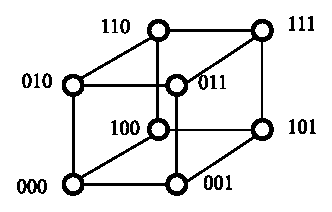
\includegraphics[width=2.111in, height=1.285in]{figures/usmanFig8}
    \caption{Hypercube topology}
    \label{fig:ch-ned-lang:hypercube-topology}
  \end{center}
\end{figure}


The hypercube topology\index{topology!hypercube} template is the
following (it can be placed into a separate file, e.g \ttt{hypercube.ned}):


\begin{Verbatim}[commandchars=\\\{\}]
\tbf{simple} Node
    \tbf{gates}:
        \tbf{out}: out[];
        \tbf{in}: in[];
\tbf{endsimple}

\tbf{module} Hypercube
    \tbf{parameters}:
        dim, nodetype;
    \tbf{submodules}:
        node: nodetype[2{\textasciicircum}dim] \tbf{like} Node
        \tbf{gatesizes}:
            out[dim], in[dim];
    \tbf{connections}:
        \tbf{for} i=0..2^dim-1, j=0..dim-1 \tbf{do}
            node[i].out[j] --> node[i # 2^j].in[j]; // # is bitwise XOR
        \tbf{endfor};
\tbf{endmodule}
\end{Verbatim}



When you create an actual hypercube, you substitute the name
of an existing module type (e.g. \ttt{"Hypercube\_PE"}) for the nodetype
parameter. The module type implements the algorithm the user
wants to simulate and it must have the same gates that the Node
type has. The topology template code can be used through importing
the file:


\begin{Verbatim}[commandchars=\\\{\}]
\tbf{import} "hypercube.ned";

\tbf{simple} Hypercube_PE
    \tbf{gates}: \tbf{out}: out[]; \tbf{in}: in[];
\tbf{endsimple}

\tbf{network} hypercube: Hypercube
    \tbf{parameters}:
        dim = 4,
        nodetype = "Hypercube_PE";
\tbf{endnetwork}
\end{Verbatim}



If you put the nodetype parameter to the ini file, you can use the
same simulation model to test e.g. several routing algorithms in a
hypercube, each algorithm implemented with a different
simple module type -- you just have to supply
different values to nodetype, such as \ttt{"WormholeRoutingNode"},
\ttt{"DeflectionRoutingNode"}, etc.






\section{GNED -- Graphical NED Editor}

\index{ned!graphical interface}

The GNED editor allows you to design compound modules graphically.
GNED works with NED files -- it doesn't use any nasty internal file
format. You can load any of your existing NED files, edit the compound
modules in it graphically and then save the file back. The rest of the
stuff in the NED file (simple modules, channels, networks etc.) will
survive the operation. GNED puts all graphics-related data into
display strings.


GNED works by parsing your NED file into an internal data structure,
and regenerating the NED text when you save the file. One consequence
of this is that indentation will be ``canonized''
-- hopefully you consider this fact as a plus and not as a minus.
Comments in the original NED are preserved -- the parser associates
them with the NED elements they belong to, so comments won't
be messed up even if you edit the graphical representation to
death by removing/adding submodules, gates, parameters, connections,
etc.

GNED is now a fully two-way visual tool. While editing the graphics,
you can always switch to NED source view, edit in there and switch
back to graphics. Your changes in the NED source will be immediately
backparsed to graphics; in fact, the graphics will be totally
reconstructed from the NED source and the display strings in
it.

GNED is still under development. There are some missing functions
and bugs, but overall it should be fairly reliable. See the TODO
file in the GNED source directory for problems and missing features.


\tbf{Comment parsing:}


It is useful to know how exactly GNED identifies the comments
in the NED file. The following (maybe a bit long) NED code should
explain it:

\begin{verbatim}
// ---------------------------------------------------------------
// File: sample.ned
//
// This is a file comment. File comments reach from the top of
// the file till the last blank line above the first code line.
// ---------------------------------------------------------------
//

// The file comment can also contain blank lines, so this is
// still part of the above file comment.
//
// Module1 --
//
// This is a banner comment for the Module1 declaration below.
// Banner comments can be multi-line, but they are not supposed
// to contain blank lines. (Otherwise the lines above the blank
// one will be taken as part of a file comment or trailing comment.)
//
module Module1
    submodules: // and this is right-comment
        // This is another banner comment, for the submodule
        submod1: Module;
            display: "p=120,108;b=96,72,rect";
            connections:
                out --> submod1.in; // Right-comments can also be
                                    // multi-line.
endmodule

// Finally, this is a trailing comment, belonging to the above
// module. It may contain blank lines. Trailing comments are
// mostly used to put separator lines into the file, like this:
// --------------------------------------------------------------
// Module2 --
//
// an empty module
//
module Module2
endmodule
\end{verbatim}


\tbf{Key/mouse bindings:}

\index{gned!mouse bindings}

In graphics view, there are two editing modes: draw and select/mode.
The mouse bindings are the following:


\begin{longtable}{|p{7cm}|p{7cm}|}
\hline
% ROW 1
\tabheadcol
\tbf{Mouse} & \tbf{Effect}\\\hline
\multicolumn{2}{|c|}{\tbf{In \textit{draw} mode:}} \\
\hline
% ROW 3
Drag out a rectangle in empty area: &  create new submodule \\\hline
% ROW 4
Drag from one submodule to another: &  create new connection \\\hline
% ROW 5
Click in empty area: & switch to select/move mode \\\hline
\multicolumn{2}{|c|}{\tbf{In \textit{select/move} mode:}} \\\hline
% ROW 7
Click submodule/connection: & select it\\\hline
% ROW 8
Ctrl-click submodule/conn.: & add to selection \\\hline
% ROW 9
Click in empty area: & clear selection\\\hline
% ROW 10
Drag a selected object: & move selected objects \\\hline
% ROW 11
Drag submodule or connection: & move it \\\hline
% ROW 12
Drag either end of connection: & move that end \\\hline
% ROW 13
Drag corner of (sub)module: & resize module\\\hline
% ROW 14
Drag starting in empty area: & select enclosed submodules/connections \\\hline
% ROW 15
\textit{Del} key & delete selected objects \\\hline
\multicolumn{2}{|c|}{\tbf{Both editing modes:}} \\\hline
% ROW 17
Right-click on module/submodule/con\-nec\-tion: & popup menu \\\hline
% ROW 18
Double-click on submodule: & go into submodule \\\hline
% ROW 19
Click name label & edit name \\\hline
% ROW 20
Drag\&drop module type from the tree view to the canvas &
create a submodule of that type \\\hline
\end{longtable}



%%% Local Variables:
%%% mode: latex
%%% TeX-master: "usman"
%%% End:
